% Provenance (never printed): see sources/outline_sources.md (Year 2: monsoons; El Niño--Southern
% Oscillation; the North Atlantic Oscillation; ocean--atmosphere coupling). Definitions after the
% IPCC AR6 glossary, the NOAA CPC ENSO FAQ and NAO pages, the NWS glossary and the IMD monsoon
% FAQ; indices from the CPC data files (data/derived/bachelor-2-{oni,oni-table,roni,nino34,nao});
% figures from figdata/bachelor-2/climvar.py; values of the examples, exercises and problem
% computed in the Book 4 scratch calculator calc/ch23.py.
\chapter{Klimaatvariabiliteit}\label{ch:b2:climate-variability}

In september 2026 was het zeeoppervlak in de centrale equatoriale Stille Oceaan gemiddeld \qty{29.27}{\celsius},
waar de gebruikelijke septemberwaarde \qty{26.71}{\celsius} is; verder naar het oosten waren delen van de oceaan
meer dan \qty{4}{\celsius} warmer dan gewoonlijk, en weervoorspellers schatten de kans op meer dan vier op vijf
dat de gebeurtenis tegen het einde van het jaar elke El~Niño sinds 1950 zou overtreffen. De eerdere
recordgebeurtenissen, in 1982, 1997 en 2015, verbleekten en doodden koralen, zetten tropische bossen in brand
en brachten hittegolven; de ansjovisvangst van Peru daalt sterk wanneer zulk warm water blijft hangen. De
oceaan en de atmosfeer van de tropische Stille Oceaan waren omgeslagen, zoals ze om de paar jaar doen, en de
omslag reikte ver voorbij de Stille Oceaan. Dit
hoofdstuk beschrijft zulke schommelingen van het klimaat, de \omterm{def:b2:climate-variability:monsoon}{moessons}, El~Niño en La~Niña, de \omterm{def:b2:climate-variability:nao}{Noord-Atlantische
Oscillatie}, en wat de oceaan tot hun geheugen maakt.
% ledger: data:b4-nino34, cpc:edd-2026-10, thirumalai24:bjerknes, cheung26:peru

\begin{recall}
\textbf{Uit de schoolboeken}: weer en klimaat; de temperatuuranomalie; de menglaag,
de thermocline en opwelling; de klimaatterugkoppeling. \textbf{Uit Boek~3}: de
Hadley-cellen, de passaatwinden, de intertropische convergentiezone en haar seizoensverschuiving, de
Walkercirculatie, opwelling langs de kust. \textbf{Uit \cref{ch:b2:weather-systems}}: de straalstroom,
\omterm{def:b2:weather-systems:rossby}{Rossby-golven}, \omterm{def:b2:weather-systems:cyclones}{extratropische cyclonen} en blokkering. \textbf{Uit de natuurkundeboeken}: warmtecapaciteit
en de eerste hoofdwet van de thermodynamica.
\end{recall}

\section{Variabiliteit en haar maten}\label{sec:b2:climate-variability:measures}

Het weer verandert van dag tot dag; het klimaat, de statistiek van het weer, verandert ook, van het ene seizoen
of het ene jaar op het volgende, zelfs wanneer er buiten het klimaatsysteem niets verandert. Een deel van die
variabiliteit is ruis, maar veel ervan is georganiseerd in enkele terugkerende patronen, met hun eigen
geografie en hun eigen tijdschalen.

\begin{definition}[Modus van klimaatvariabiliteit; klimaatindex; klimatologie]\label{def:b2:climate-variability:modes}
Een \emph{modus van klimaatvariabiliteit}\index{modus van klimaatvariabiliteit} is een terugkerend patroon van
natuurlijke variabiliteit van het klimaatsysteem, met een eigen ruimtelijk patroon, seizoensgebondenheid en eigen
tijdschalen, dat voortkomt uit de dynamica van de atmosfeer of uit de koppeling van de oceaan en de
atmosfeer. Een \emph{klimaatindex}\index{klimaatindex} is een tijdreeks, opgebouwd uit
klimaatvariabelen, die de toestand van zo'n patroon samenvat, bijvoorbeeld het verschil in luchtdruk op zeeniveau
tussen IJsland en de Azoren. De \emph{klimatologie}\index{klimatologie} van een variabele
is haar gemiddelde over een referentieperiode, berekend voor elke kalendermaand of elk seizoen; de
standaardreferentieperiode is 30 jaar lang, momenteel 1991--2020.
\end{definition}
% ledger: ipccgl:modes, ipccgl:index, wmo:normal-30yr

Veel modi worden aangedreven door processen binnen het klimaatsysteem: ze maken deel uit van zijn
interne variabiliteit. Omdat ze met hun eigen tijdschalen terugkeren, zijn ze een bron van
voorspelbaarheid buiten het bereik van weersverwachtingen, van weken tot decennia. Indices maken ze
meetbaar. Een index wordt berekend uit anomalieën, zoals in de schoolboeken, en
afgevlakt.
% ledger: ipccgl:modes

\begin{method}[Van waarnemingen naar een index]\label{met:b2:climate-variability:index}
\begin{enumerate}
  \item Bereken de \omterm{def:b2:climate-variability:modes}{klimatologie}: het gemiddelde van de variabele voor elke kalendermaand over de
        referentieperiode.
  \item Trek haar af: de anomalie van elke maand is haar waarde min de \omterm{def:b2:climate-variability:modes}{klimatologie} van die maand.
        De seizoenscyclus verdwijnt; wat overblijft, is de variabiliteit.
  \item Vlak de anomalieën af met een lopend gemiddelde, het gemiddelde van $n$ opeenvolgende waarden gecentreerd op
        elke maand, om de schommelingen te verwijderen die korter zijn dan het patroon dat ons interesseert.
  \item Als de index met andere moet worden vergeleken, deel dan door zijn standaardafwijking: de index
        is dan gestandaardiseerd, in eenheden van standaardafwijkingen.
\end{enumerate}
\end{method}

\begin{example}[Een anomalie]\label{ex:b2:climate-variability:anomaly}
De gemiddelde temperatuur van het zeeoppervlak van de centrale equatoriale Stille Oceaan tussen \ang{5}~NB en
\ang{5}~ZB, \ang{170}~WL en \ang{120}~WL was \qty{29.27}{\celsius} in september 2026. Haar
septemberklimatologie is \qty{26.71}{\celsius}, dus de anomalie was $29.27 - 26.71 = \qty{2.56}{\celsius}$.
In september 1997 had dezelfde oceaan \qty{28.79}{\celsius} tegen \qty{26.73}{\celsius}, een
anomalie van \qty{2.06}{\celsius}. De twee klimatologieën verschillen een beetje omdat de
referentieperiode om de vijf jaar wordt verschoven: de oceaan zelf is opgewarmd.
% ledger: data:b4-nino34, cpc:oni-def
\end{example}

\section{Moessons}\label{sec:b2:climate-variability:monsoons}

\begin{definition}[Moesson]\label{def:b2:climate-variability:monsoon}
Een \emph{moesson}\index{moesson} is een thermisch aangedreven wind, ontstaan door de verschillende opwarming van
een landmassa en de aangrenzende oceaan, die met de seizoenen van richting omkeert, samen met
de seizoensomkering van de neerslag die hij brengt.
\end{definition}
% ledger: nws4:monsoon, ipccgl:monsoon

Op het land blijft de warmte van de zomerzon in een dunne laag dicht bij het oppervlak, terwijl de zee
dezelfde warmte door haar menglaag van tientallen meters diep omlaag mengt en veel minder opwarmt. De lucht boven
het land warmt meer op, haar druk aan het oppervlak daalt, en vochtige lucht stroomt vanuit zee binnen, stijgt, koelt af en
geeft regen; in de hoogte keert de lucht terug naar zee. In de winter is het land het koudere oppervlak en keert de circulatie
om. Samen vormen de \omterm{def:b2:climate-variability:monsoon}{moessons} van de planeet één mondiaal patroon dat de jaarlijkse
cyclus van tropische en subtropische regen beheerst; zijn domein wordt gedefinieerd als de gebieden waar de gemiddelde regen
van de plaatselijke zomer die van de winter met meer dan \qty{2.5}{mm} per dag overtreft.
% ledger: nws4:monsoon, ipccgl:monsoon

\begin{omfigure}
\centering
\begin{tikzpicture}[font=\scriptsize, >=Stealth]
\foreach \col/\title in {0/{a\enspace zomer}, 7.2/{b\enspace winter}} {
  \begin{scope}[shift={(\col,0)}]
  \node[anchor=south west] at (0,3.0) {\textbf{\title}};
  \fill[ocBlue!18] (0,0) rectangle (3,0.35);
  \fill[brown!35] (3,0) -- (6.4,0) -- (6.4,0.5) -- (3,0.35) -- cycle;
  \node at (1.5,0.17) {zee};
  \node at (4.7,0.2) {land};
  \end{scope}
}
% summer: low over the land, inflow from the sea, rising air and rain
\node[font=\small\bfseries, ocBlue] at (0.45,0.62) {H};
\node[font=\small\bfseries, ocRed] at (4.8,0.78) {L};
\node[ocRed, anchor=west] at (5.35,0.78) {heet};
\draw[->, thick] (1.0,0.98) -- (4.2,1.02);
\node at (2.4,0.66) {vochtige lucht van zee};
\draw[->, thick] (4.8,1.15) -- (4.8,2.55);
\draw[->, thick] (4.45,2.8) -- (1.75,2.8);
\draw[->, thick] (1.4,2.6) -- (1.4,1.25);
\fill[black!15, draw=black!40] (4.0,1.9) .. controls (4.0,2.55) and (5.6,2.55) .. (5.6,1.9) -- cycle;
\foreach \x in {4.25,4.5,5.1,5.35} {\draw[ocBlue, dashed] (\x,1.85) -- (\x-0.1,1.2);}
\node[anchor=west] at (5.65,2.1) {regen};
% winter: high over the land, dry outflow to the sea
\begin{scope}[shift={(7.2,0)}]
\node[font=\small\bfseries, ocRed] at (0.45,0.62) {L};
\node[font=\small\bfseries, ocBlue] at (4.8,0.78) {H};
\node[ocBlue, anchor=west] at (5.35,0.78) {koud};
\draw[->, thick] (4.2,1.02) -- (1.0,0.98);
\node at (2.4,0.66) {droge lucht van het land};
\draw[->, thick] (1.4,1.25) -- (1.4,2.6);
\draw[->, thick] (1.75,2.8) -- (4.45,2.8);
\draw[->, thick] (4.8,2.55) -- (4.8,1.15);
\end{scope}
\end{tikzpicture}
\par\smallskip{\small De \omterm{def:b2:climate-variability:monsoon}{moesson} als land--zeecirculatie (schematische doorsnede, niet op schaal): in
de zomer is het land het warmere oppervlak, met lage druk aan de grond, instroming van vochtige lucht vanuit
zee, stijgende lucht en regen; in de winter keert de circulatie om en is de landwind droog.}
\end{omfigure}
% ledger: nws4:monsoon, imd:heat-low

De \omterm{def:b2:climate-variability:monsoon}{moesson} van Zuid- en Zuidoost-Azië begint eind mei of begin juni, trekt naar het
noordoosten en eindigt eind september of begin oktober. Daarvoor warmen de landen rond de
Arabische Zee op: in juni stuurt het oppervlak ongeveer \qty{160}{W/m^2} warmte de lucht in boven
het droge noordwesten van India, Pakistan en het Midden-Oosten, en daar vormt zich een ondiepe hittedepressie,
die maar tot ongeveer \qty{1.5}{km} reikt, met weinig regen; een zwakke hittedepressie, zoals in het droogtejaar
1987, betekent een zwakke aantrekking op de vochtige lucht van de oceaan. Vanuit haar loopt een langgerekte trog van lage druk, de
moessontrog, naar de kop van de Golf van Bengalen; zijn noord--zuidschommelingen brengen de actieve
perioden en de onderbrekingen van het seizoen. Over heel India bedraagt de regen van juni tot september gemiddeld
\qty{88}{cm}, met een standaardafwijking van \qty{9}{cm}, ongeveer \qty{10}{\percent}: een seizoen binnen
\qty{10}{\percent} van het langjarig gemiddelde heet normaal. Aan de kust van Kerala, waar de
nationale weerdienst het begin van de \omterm{def:b2:climate-variability:monsoon}{moesson} uitroept op grond van de regenval van veertien stations,
de winden en de door satellieten gemeten uitgaande infraroodstraling, bedraagt de gemiddelde regenval
\qty{556}{mm} in juni en \qty{659}{mm} in juli.
% ledger: ipccgl:monsoon, imd:heat-low, imd:lpa, imd:onset

De West-Afrikaanse \omterm{def:b2:climate-variability:monsoon}{moesson} brengt vochtige zuidwestenwinden vanuit de Golf van Guinee, die van mei tot september
noordwaarts oprukken; zijn regen piekt rond \ang{12}~NB eind augustus en in september en
trekt vanaf oktober terug.
% ledger: ipccgl:monsoon

Een \omterm{def:b2:climate-variability:monsoon}{moesson} is regelmatig in zijn timing, onregelmatig in zijn hoeveelheid, en de schommelingen van jaar tot jaar van de
tropische Stille Oceaan behoren tot de oorzaken. El~Niño-jaren laten India vaak met een regentekort achter: de
droogten van 1904, 1972 en 1987 kwamen met El~Niño. Het verband is niet zeker: in 1997 viel een sterke
El~Niño samen met een positieve fase van de Indische Oceaan-dipool, een modus die verderop aan bod komt, en India
had een bijna normale \omterm{def:b2:climate-variability:monsoon}{moesson}.
% ledger: narang24:enso-monsoon, ipccgl:other-modes

\section{El Niño en de Zuidelijke Oscillatie}\label{sec:b2:climate-variability:enso}

Boek~3 beschreef de Walkercirculatie: lucht die opstijgt boven de warme westelijke Stille Oceaan,
in de hoogte naar het oosten stroomt, daalt boven de koele oostelijke Stille Oceaan en met de
passaatwinden naar het westen terugkeert. In de oceaan eronder stapelen de passaatwinden warm water op in het westen, waar de thermocline
diep ligt, en trekken ze koud water omhoog langs de evenaar in het oosten, waar ze ondiep ligt. Deze toestand ligt niet
vast.

\begin{definition}[El Niño--Zuidelijke Oscillatie; El Niño; La Niña; Zuidelijke Oscillatie]\label{def:b2:climate-variability:enso}
De \emph{El Niño--Zuidelijke Oscillatie}\index{El Niño--Zuidelijke Oscillatie} (ENSO) is de
gekoppelde oceaan--atmosfeermodus van de tropische Stille Oceaan: samenhangende variaties van jaar tot jaar van de
temperatuur van het zeeoppervlak, de convectieve neerslag, de druk aan het oppervlak en de circulatie langs
de equatoriale Stille Oceaan, met voorkeurstijdschalen van twee tot ongeveer zeven jaar. \emph{El
Niño}\index{El Niño} is zijn warme fase, een opwarming van het zeeoppervlak van de centrale en
oost-centrale equatoriale Stille Oceaan; \emph{La Niña}\index{La Niña} is zijn koude fase, een afkoeling van
hetzelfde gebied. De \emph{Zuidelijke Oscillatie}\index{Zuidelijke Oscillatie} is zijn atmosferische deel,
een wip van luchtdruk aan het oppervlak tussen de westelijke en de oostelijke tropische Stille Oceaan: tijdens El~Niño
is de druk hoger dan gemiddeld boven Indonesië en de westelijke Stille Oceaan en lager boven de
oostelijke Stille Oceaan, en omgekeerd tijdens La~Niña.
\end{definition}
% ledger: cpc:enso-faq, cpc:enso-faq-so, ipccgl:enso

Tijdens El~Niño verzwakken de oostelijke passaatwinden langs de evenaar, en in het westen kunnen de
winden laag bij de grond zelfs uit het westen waaien; het warme water van het westen verspreidt zich naar het oosten, en de diepe
convectie en haar regen volgen het, waardoor Indonesië en Noord-Australië droger worden. Het zeeoppervlak
van de oost-centrale Stille Oceaan is doorgaans \qtyrange{1.5}{2.5}{\celsius} warmer dan gemiddeld, en
de thermocline ligt daar op \qtyrange{150}{175}{m}, dieper dan gewoonlijk. Tijdens La~Niña worden de
passaatwinden over het hele bekken sterker, is het zeeoppervlak \qtyrange{1}{2}{\celsius} kouder dan
gemiddeld, en stijgt de thermocline in het oosten tot \qtyrange{50}{100}{m}. De Walkercirculatie
verzwakt tijdens El~Niño en wordt sterker tijdens La~Niña. Episodes keren doorgaans om de drie tot
vijf jaar terug, met tussenpozen die van twee tot zeven jaar hebben gevarieerd; een El~Niño duurt doorgaans negen tot
twaalf maanden, een La~Niña één tot drie jaar. Beide ontwikkelen zich meestal tussen maart en juni,
pieken tussen december en april en verzwakken tussen mei en juli; hun effecten zijn het sterkst
van december tot april, wanneer het equatoriale zeeoppervlak het warmst is.
% ledger: cpc:enso-faq-features, cpc:enso-faq-timing

\begin{omfigure}
\centering
\begin{tikzpicture}[font=\scriptsize, >=Stealth, x=1cm, y=0.8cm]
\foreach \row/\title/\tw/\te/\rx/\cwidth in {
    0/{a\enspace neutraal}/1.15/0.35/1.6/1.0,
    -4.6/{b\enspace El Niño}/0.95/0.85/5.6/1.4,
    -9.2/{c\enspace La Niña}/1.3/0.18/1.0/0.8} {
  \begin{scope}[shift={(0,\row)}]
  \node[anchor=south west] at (0,2.55) {\textbf{\title}};
  % ocean: warm layer above the thermocline
  \fill[ocBlue!20] (0,-1.5) rectangle (11,0);
  \fill[omWarm!25] (0,0) -- (0,-\tw) .. controls (4,-\tw) and (7,-\te) .. (11,-\te) -- (11,0) -- cycle;
  \draw[thick, ocBlue!70!black] (0,-\tw) .. controls (4,-\tw) and (7,-\te) .. (11,-\te);
  \draw (0,0) -- (11,0);
  % convection and Walker cell
  \fill[black!15, draw=black!40] ({\rx-\cwidth/2},0.5) .. controls ({\rx-\cwidth/2},2.1) and ({\rx+\cwidth/2},2.1) .. ({\rx+\cwidth/2},0.5) -- cycle;
  \draw[->, thick] (\rx,0.55) -- (\rx,2.15);
  \draw[->, thick] ({\rx+0.4},2.3) -- (9.6,2.3);
  \draw[->, thick] (10.0,2.1) -- (10.0,0.5);
  \draw[->, thick] (9.6,0.3) -- ({\rx+0.7},0.3);
  \end{scope}
}
\node[anchor=west] at (2.3,1.4) {stijgende lucht, regen};
\node[anchor=east] at (9.9,1.4) {dalende lucht};
\node at (6.0,0.55) {passaatwinden};
\node[anchor=west, ocBlue!70!black] at (7.6,-0.95) {thermocline};
\node[anchor=east] at (4.8,-4.6+1.4) {regen trekt naar het oosten};
\node at (8.2,-4.6+0.55) {zwakke passaatwinden};
\node at (6.0,-9.2+0.55) {sterke passaatwinden};
\node[ocBlue!70!black, align=center] at (9.6,-9.2-0.8) {koud water\\dicht bij het oppervlak};
\node[anchor=north west] at (0,-9.2-1.55) {west (Indonesië)};
\node[anchor=north east] at (11,-9.2-1.55) {oost (Zuid-Amerika)};
\end{tikzpicture}
\par\smallskip{\small De equatoriale Stille Oceaan langs de evenaar in de drie fasen van ENSO
(schematisch, niet op schaal): de Walkercirculatie boven, de warme bovenlaag en de
thermocline onder. Tijdens El~Niño verzwakken de passaatwinden, verspreiden het warme water en de regen zich naar het oosten
en zakt de thermocline in het oosten tot \qtyrange{150}{175}{m}; tijdens La~Niña worden de passaten
sterker en stijgt de thermocline in het oosten tot \qtyrange{50}{100}{m}.}
\end{omfigure}
% ledger: cpc:enso-faq-features, climategov:walker

De namen komen uit verschillende eeuwen en verschillende wetenschappen. Vissers aan de kust van
Zuid-Amerika merkten rond Kerstmis een opwarming van hun kustwateren op die de visserij
verstoorde, en noemden haar El~Niño, het jongetje. Sir Gilbert Walker ontdekte de \omterm{def:b2:climate-variability:enso}{Zuidelijke
Oscillatie} in de atmosfeer, zonder haar met de oceaan te verbinden. Pas eind jaren 1960 zagen Jacob Bjerknes en anderen in dat de
twee één verschijnsel waren. De termen La~Niña en neutraal raakten in de jaren 1980 ingeburgerd.
% ledger: climategov:enso-history, ipccgl:enso

\begin{history}[Het jongetje van de vissers]
\begin{minipage}[t]{0.54\linewidth}\vspace{0pt}
Voor de droge kust van Peru is het koude water dat de winden langs de kust omhoog trekken, rijk aan
voedingsstoffen en voedt het een productieve visserij. De vissers kenden een opwarming die rond
Kerstmis kwam, wanneer de vis schaars werd, en gaven haar de naam van het kind van het seizoen. De
ansjovisvangst van Peru volgt ENSO nog altijd: volgens een recente analyse maakten langdurig hoge
temperatuuranomalieën een extreem lage vangst meer dan negen keer waarschijnlijker, met een mediane daling van de
vangst van ongeveer \qty{60}{\percent}; de sterke El~Niño van 1997--98 springt eruit in de reeks.
\end{minipage}\hfill
\begin{minipage}[t]{0.42\linewidth}\vspace{0pt}
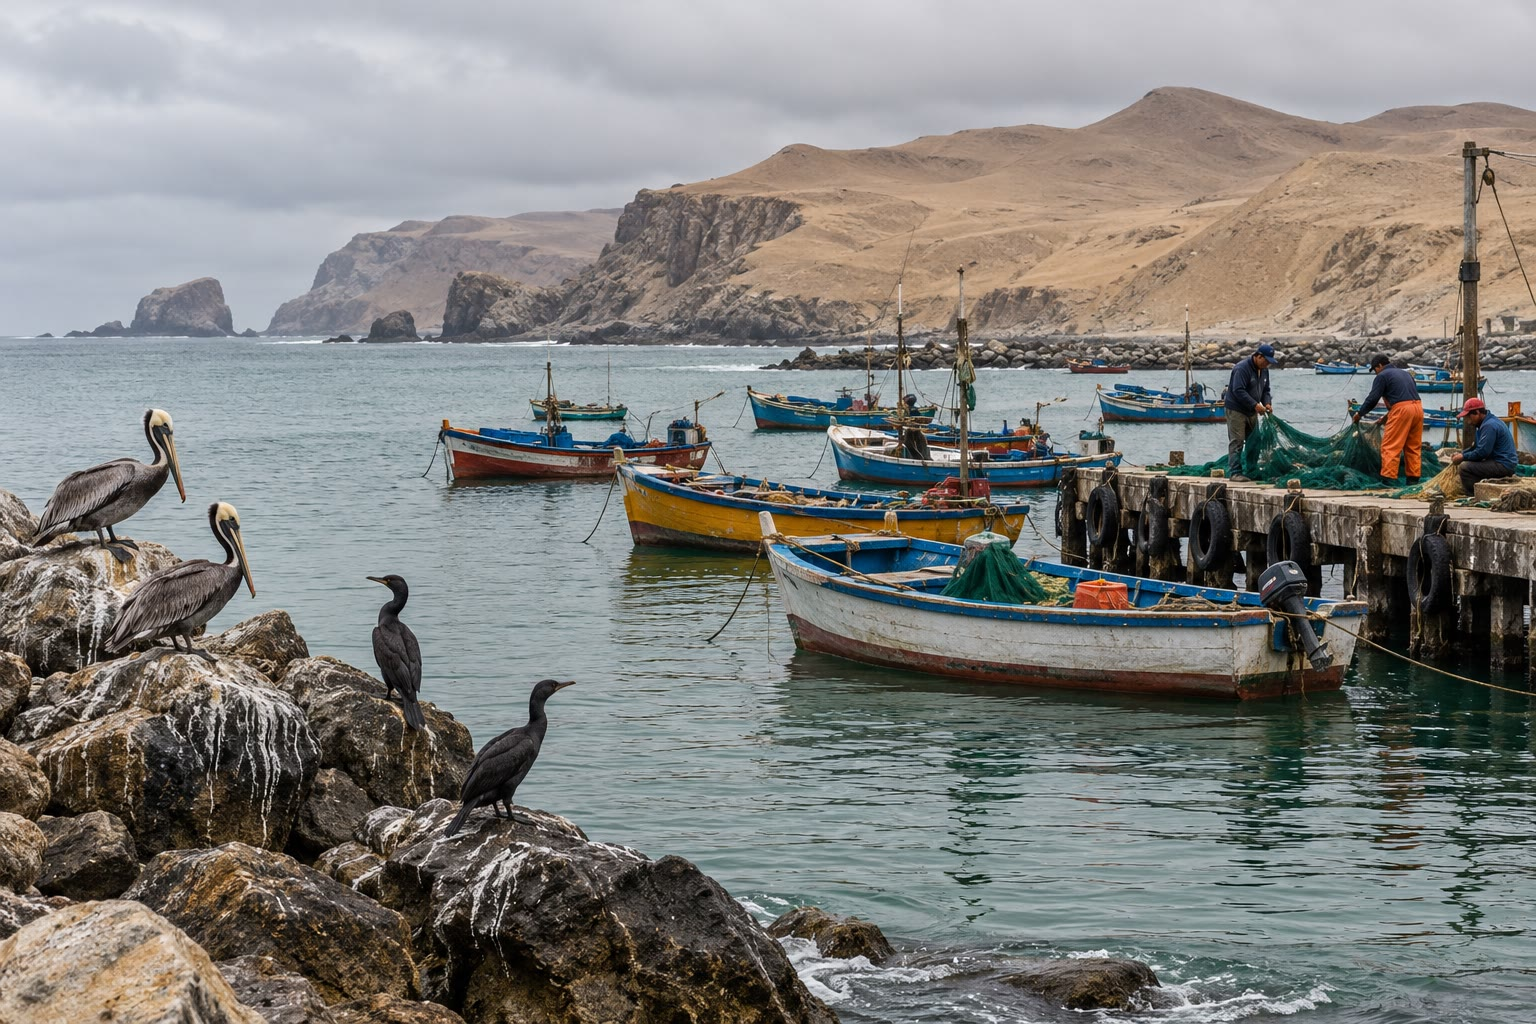
\includegraphics[width=\linewidth]{images/book4/ai/b2-fishing-harbour.jpg}

{\scriptsize Vissersboten in een haven aan een woestijnkust met koud opwellend water
(door AI gegenereerde illustratie).}
\end{minipage}
% ledger: climategov:enso-history, cheung26:peru, stewart:upwelling
\end{history}

Waarom schommelt het systeem eigenlijk? Omdat de oceaan en de atmosfeer van de equatoriale Stille Oceaan
elkaars anomalieën versterken.

\begin{definition}[Bjerknes-terugkoppeling]\label{def:b2:climate-variability:bjerknes}
De \emph{Bjerknes-terugkoppeling}\index{Bjerknes-terugkoppeling} is de positieve terugkoppeling tussen de
temperatuur van het zeeoppervlak, de winden en de oceaanstromingen van de equatoriale Stille Oceaan: een opwarming van
het oosten verzwakt het oost--westcontrast van temperatuur en druk, en dus de passaatwinden;
zwakkere passaatwinden laten het warme water van het westen naar het oosten uitvloeien en brengen minder koud water omhoog in het
oosten, wat het oosten verder opwarmt. Dezelfde lus versterkt een afkoeling.
\end{definition}
% ledger: thirumalai24:bjerknes, cpc:enso-faq-timing

\begin{omfigure}
\centering
\begin{tikzpicture}[font=\small, >=Stealth, box/.style={draw, rounded corners=2pt, fill=omDef!8,
  align=center, text width=4.3cm, minimum height=1.05cm, inner sep=3pt}]
\node[box] (a) at (0,2) {oostelijke equatoriale\\Stille Oceaan warmer\\dan gewoonlijk};
\node[box] (b) at (6.2,2) {kleiner oost--westcontrast\\van temperatuur en druk};
\node[box] (c) at (6.2,0) {zwakkere passaatwinden};
\node[box] (d) at (0,0) {warm water vloeit\\naar het oosten,\\minder koud water omhoog};
\draw[->, very thick, ocRed] (a) -- (b);
\draw[->, very thick, ocRed] (b) -- (c);
\draw[->, very thick, ocRed] (c) -- (d);
\draw[->, very thick, ocRed] (d) -- (a);
\node[ocRed, font=\bfseries] at (3.1,1) {$+$};
\end{tikzpicture}
\par\smallskip{\small De \omterm{def:b2:climate-variability:bjerknes}{Bjerknes-terugkoppeling}, getekend voor een opwarming; met elke pijl omgekeerd verdiept
dezelfde lus een afkoeling. Een positieve lus van deze soort versterkt een kleine verstoring.}
\end{omfigure}
% ledger: thirumalai24:bjerknes

Een positieve terugkoppeling verklaart hoe een anomalie groeit, niet hoe ze begint of eindigt. Volgens een gangbare verklaring
begint een El~Niño wanneer willekeurige schommelingen van de passaatwinden de equatoriale stromingen verzwakken die
het warme water in het westen houden; de warme poel verspreidt zich naar het oosten, de convectie volgt haar, de
\omterm{def:b2:climate-variability:bjerknes}{Bjerknes-terugkoppeling} neemt het over en de gebeurtenis groeit. La~Niña-gebeurtenissen worden volgens dezelfde verklaring
uitgelokt door een voorafgaande El~Niño. De eenvoudigste modellen die het systeem laten oscilleren, de
opladingsoscillator onder hen, koppelen twee grootheden: de anomalie van de temperatuur van het zeeoppervlak van de centrale
Stille Oceaan en het volume warm water in de bovenste oceaanlaag dat langs de evenaar is opgeslagen. De
temperatuuranomalie laat die voorraad leeglopen of vult hem aan via de winden die ze aandrijft, en de voorraad bereidt via de
diepte van de thermocline de volgende fase voor. \Cref{exo:b2:climate-variability:10} lost
zo'n paar vergelijkingen op.
% ledger: thirumalai24:bjerknes, stuecker25:ro

Om ENSO te volgen gebruiken de monitoringcentra indices.

\begin{definition}[Niño-3.4-index; Oceanische Niño-index]\label{def:b2:climate-variability:oni}
De \emph{Niño-3.4-index}\index{Niño-3.4-index} is de maandelijkse anomalie van de temperatuur van het
zeeoppervlak, gemiddeld over het gebied \ang{5}~NB--\ang{5}~ZB, \ang{170}~WL--\ang{120}~WL, ten opzichte van
de \omterm{def:b2:climate-variability:modes}{klimatologie} van een basisperiode van 30 jaar rond het jaar, die om de vijf jaar wordt bijgewerkt. De
\emph{Oceanische Niño-index}\index{Oceanische Niño-index} (ONI) is zijn lopend driemaandsgemiddelde. Een
El~Niño-episode (La~Niña-episode) is een reeks van minstens vijf opeenvolgende, overlappende driemaandse seizoenen
waarin de ONI op of boven \qty{+0.5}{\celsius} (op of onder \qty{-0.5}{\celsius}) ligt.
\end{definition}
% ledger: cpc:oni-def, cpc:enso-faq

De seizoenen overlappen: DJF, JFM, FMA enzovoort, elk het gemiddelde van drie maanden, elk met twee
maanden gemeen met het volgende. Een tweede index, de Zuidelijke-Oscillatie-index, volgt de atmosfeer: hij
wordt berekend uit de afwijkingen van het drukverschil tussen Tahiti en Darwin, negatief
tijdens El~Niño, positief tijdens La~Niña. Sinds februari 2026 is de officiële index om ENSO te
volgen een relatieve ONI, berekend uit de Niño-3.4-anomalie min de gemiddelde anomalie van de hele
tropische oceaan tussen \ang{20}~NB en \ang{20}~ZB, en daarna herschaald naar de amplitude van de ONI. Omdat hij
tegen de hele tropen wordt gemeten, hangt hij minder af van de keuze van de basisperiode terwijl de oceanen
opwarmen, en hangt hij beter samen met de regenval van de tropische Stille Oceaan. In september 2026 bedroeg de
relatieve anomalie van het Niño-3.4-gebied \qty{2.08}{\celsius}, tegen de \qty{2.56}{\celsius}
van \cref{ex:b2:climate-variability:anomaly}: ongeveer een halve graad van de traditionele anomalie was de
warmte van de tropische oceanen als geheel.
% ledger: cpc:enso-faq-so, pns:roni, data:b4-rnino34

\begin{omfigure}
\centering
% figdata/bachelor-2/climvar.py part oni
\begin{tikzpicture}
\begin{axis}[width=\linewidth, height=6.0cm, xmin=1950, xmax=2027, ymin=-2.4, ymax=3.0,
  xlabel={jaar}, ylabel={index (\unit{\celsius})}, tick label style={font=\scriptsize},
  label style={font=\small}, xtick={1950,1960,...,2020}, x tick label style={/pgf/number
  format/1000 sep={}}, legend style={font=\scriptsize, at={(0.5,1.02)}, anchor=south,
  draw=none, legend columns=3, /tikz/every even column/.append style={column sep=6pt}},
  legend cell align=left]
\addplot[fill=ocRed!70, draw=none, area legend] table[x=t, y=pos]
  {figdata/out/bachelor-2-climvar-oni.dat} \closedcycle;
\addlegendentry{ONI, El Niño-kant}
\addplot[fill=ocBlue!70, draw=none, area legend] table[x=t, y=neg]
  {figdata/out/bachelor-2-climvar-oni.dat} \closedcycle;
\addlegendentry{ONI, La Niña-kant}
\addplot[black, thin] table[x=t, y=roni] {figdata/out/bachelor-2-climvar-oni.dat};
\addlegendentry{relatieve ONI}
\addplot[black!60, densely dashed, domain=1950:2027, samples=2] {0.5};
\addplot[black!60, densely dashed, domain=1950:2027, samples=2] {-0.5};
\end{axis}
\end{tikzpicture}
\par\smallskip{\small De \omterm{def:b2:climate-variability:oni}{Oceanische Niño-index} van DJF 1950 tot JAS 2026 (één waarde per
driemaands seizoen, uitgezet bij de middelste maand), en de relatieve ONI, de officiële index sinds
februari 2026; gestreept: de drempels $\pm\qty{0.5}{\celsius}$. Gegevens: NOAA Climate Prediction
Center, opgehaald op 23 oktober 2026.}
\end{omfigure}
% ledger: data:b4-oni, data:b4-roni

Geteld met de vijfseizoenenregel op de tabel van het Climate Prediction Center toont de ONI 25
El~Niño- en 21 La~Niña-episodes tussen 1950 en de zomer van 2026. De sterkste El~Niño-pieken
waren \qty{2.4}{\celsius} eind 1997 en \qty{2.6}{\celsius} eind 2015. De twee indices
lopen het verst uiteen in de laatste jaren: in juli--september 2026 stond de ONI op \qty{2.2}{\celsius} en
de relatieve index op \qty{1.7}{\celsius}.
% ledger: data:b4-oni, data:b4-roni

\begin{dated}{2026}
In zijn bespreking van 8 oktober 2026 handhaafde het Climate Prediction Center zijn El~Niño-advies: de
relatieve Niño-3.4-anomalie had in september \qty{+2.1}{\celsius} bereikt, delen van de oostelijke
equatoriale Stille Oceaan lagen meer dan \qty{4}{\celsius} boven het gemiddelde, het water op diepte in het oosten
meer dan \qty{10}{\celsius}, en de indices van de \omterm{def:b2:climate-variability:enso}{Zuidelijke Oscillatie} waren significant
negatief. Een
sterke tot zeer sterke El~Niño werd waarschijnlijk geacht tot januari--maart 2027, en de kans dat
de relatieve index \qty{2.5}{\celsius} zou overschrijden, voorbij elke gebeurtenis sinds 1950, werd op
\qty{83}{\percent} gesteld voor oktober--december.
% ledger: cpc:edd-2026-10, data:b4-rnino34
\end{dated}

\section{De Noord-Atlantische Oscillatie en teleconnecties}\label{sec:b2:climate-variability:nao}

\begin{definition}[Noord-Atlantische Oscillatie]\label{def:b2:climate-variability:nao}
De \emph{Noord-Atlantische Oscillatie}\index{Noord-Atlantische Oscillatie} (NAO) is de belangrijkste modus
van atmosferische variabiliteit boven de Noord-Atlantische Oceaan: een wip van de luchtdruk op zeeniveau tussen de
IJslandse depressie en het Azorenhoog. Haar index is positief wanneer beide sterker zijn dan gemiddeld, zodat
het drukverschil ertussen groot is, en negatief wanneer beide zwakker zijn.
\end{definition}
% ledger: ipccgl:other-modes, climategov:nao, cpc:nao-teledoc

De NAO stuurt de westenwinden van het vorige hoofdstuk. In haar positieve fase drijft het grotere
drukverschil een sterkere Atlantische straalstroom aan en verschuift het de stormbaan naar het noorden: Noord-Europa
heeft een stormachtigere, nattere en zachtere winter, Zuid-Europa een drogere, het oosten van Noord-Amerika
minder uitbraken van koude lucht, en Groenland een koudere winter. De negatieve fase keert deze
anomalieën om. Eind achttiende eeuw merkte een zendeling al op dat zachte winters in
Groenland samengingen met strenge in Denemarken, en omgekeerd.
% ledger: climategov:nao, cpc:nao-teledoc

De NAO is in elk seizoen een van de opvallendste patronen van de atmosfeer, en ze is
sterk gecorreleerd met een andere modus, de Arctische Oscillatie. Ze varieert ook over decennia: de negatieve fase overheerste
van het midden van de jaren 1950 tot de winter van 1978--79, en de positieve fase van 1979--80 tot 1994--95.
% ledger: cpc:nao-teledoc, climategov:nao

\begin{omfigure}
\centering
% figdata/bachelor-2/climvar.py part nao
\begin{tikzpicture}
\begin{axis}[width=\linewidth, height=5.4cm, xmin=1950, xmax=2027, ymin=-1.9, ymax=1.9,
  ytick={-1,0,1},
  xlabel={winter (jaar van zijn januari)}, ylabel={NAO-index (DJF-gemiddelde)},
  tick label style={font=\scriptsize}, label style={font=\small}, xtick={1950,1960,...,2020},
  x tick label style={/pgf/number format/1000 sep={}}, legend style={font=\scriptsize,
  at={(0.5,1.02)}, anchor=south, draw=none, legend columns=2,
  /tikz/every even column/.append style={column sep=6pt}},
  legend cell align=left, unbounded coords=jump]
\addplot[ybar, bar width=0.6, fill=omDef!55, draw=none, area legend] table[x=year, y=nao]
  {figdata/out/bachelor-2-climvar-nao.dat};
\addlegendentry{wintergemiddelde}
\addplot[ocRed, thick] table[x=year, y=run5] {figdata/out/bachelor-2-climvar-nao.dat};
\addlegendentry{lopend gemiddelde over 5 winters}
\end{axis}
\end{tikzpicture}
\par\smallskip{\small Het wintergemiddelde (december--februari) van de maandelijkse NAO-index van het NOAA
Climate Prediction Center, 1951--2026, in standaardafwijkingen, met zijn gecentreerd lopend gemiddelde over vijf
winters. De laagste winter is 2010 ($-1.67$), de hoogste 2015 ($+1.66$).}
\end{omfigure}
% ledger: data:b4-nao, cpc:nao-teledoc

De NAO, ENSO en de andere modi werken ver van de plaats waar ze worden gemeten.

\begin{definition}[Teleconnectie]\label{def:b2:climate-variability:teleconnection}
Een \emph{teleconnectie}\index{teleconnectie} is een samenhang tussen klimaatvariabelen op
ver van elkaar verwijderde, vaste plaatsen, verbonden door fysische processen langs wegen in de atmosfeer of de
oceaan, zoals reeksen \omterm{def:b2:weather-systems:rossby}{Rossby-golven}, verschuivingen van de straalstroom en de stormbanen, of veranderingen
van de Walkercirculatie.
\end{definition}
% ledger: ipccgl:teleconnection

Tijdens El~Niño verandert de regenval van de tropen van Indonesië tot Zuid-Amerika, ongeveer halverwege
rond de wereld, en vanuit de tropen reizen de anomalieën naar de middelbare breedten langs de wegen
van de definitie; de Indiase \omterm{def:b2:climate-variability:monsoon}{moesson} van de vorige paragraaf is een van hun eindpunten. In elke oceaan zijn andere modi
benoemd: de Indische Oceaan-dipool, een oost--westwip van de temperatuur van het
zeeoppervlak in de tropische Indische Oceaan, waarvan de positieve fase de zee voor Sumatra en Java afkoelt
en voor Somalië opwarmt, die zich in de noordelijke zomer ontwikkelt, in de herfst tot rijping komt, en
de regen van Australië, Zuidoost-Azië en Oost-Afrika verandert; de Zuidelijke Annulaire Modus, de veranderingen van
sterkte en breedteligging van de westenwindgordel rond Antarctica; en de decadale variabiliteit van de
Stille Oceaan, trager dan ENSO.
% ledger: cpc:enso-faq, ipccgl:other-modes, ipccgl:teleconnection, narang24:enso-monsoon

\section{De oceaan als geheugen}\label{sec:b2:climate-variability:memory}

\Cref{ch:b2:weather-systems} vond dat de atmosfeer haar weer binnen ongeveer twee weken vergeet.
Een klimaatanomalie die een seizoen duurt, moet ergens worden opgeslagen, en de voor de hand liggende opslag is de menglaag
van de oceaan: een diepere menglaag bevat meer warmte en heeft meer thermische traagheid. Het eenvoudigste model behandelt de
anomalie als een reservoir dat warmte lekt naar de atmosfeer.
% ledger: shi22:memory

\begin{proposition}[Dempingstijd van een anomalie in de menglaag]\label{prop:b2:climate-variability:damping}
Laat een menglaag met diepte $h$, dichtheid $\rho$ en soortelijke warmte $c_p$ een temperatuuranomalie
$T'$ dragen, en laat het oppervlak per oppervlakte-eenheid een extra warmteflux $\alpha T'$ aan de atmosfeer verliezen,
met $\alpha > 0$. Dan geldt, zonder andere forcering,
\[
  T'(t) = T'(0)\,\mathrm{e}^{-t/\tau}, \qquad \tau = \frac{\rho\,c_p\,h}{\alpha} .
\]
\end{proposition}

\begin{proof}
De warmte-inhoud van de anomalie per oppervlakte-eenheid is $\rho c_p h T'$; de eerste hoofdwet geeft $\rho c_p h
\,\mathrm{d}T'/\mathrm{d}t = -\alpha T'$, een lineaire vergelijking waarvan de oplossing het exponentiële
verval met de tijdconstante $\tau$ is.
\end{proof}
% ledger: shi22:memory

\begin{example}[Het geheugen van een oceaan op middelbare breedte]\label{ex:b2:climate-variability:tau}
Boven de oceanen van de middelbare breedten reageert de warmteflux aan het oppervlak op een anomalie van de temperatuur van het
zeeoppervlak met een gemiddelde $\alpha = \qty{16.1}{W.m^{-2}.K^{-1}}$. Voor een menglaag
van \qty{50}{m} diep, met $\rho = \qty{1025}{kg/m^3}$ en $c_p = \qty{3992}{J.kg^{-1}.K^{-1}}$, is
$\tau = 1025 \times 3992 \times 50/16.1 = \qty{1.27e7}{s} = \qty{147}{\day}$, bijna vijf
maanden; een laag van \qty{100}{m} diep onthoudt twee keer zo lang.
\end{example}
% ledger: wang24:shff, noaa:seawater-1025, teos10:cp0

Echte anomalieën worden ook elke dag geforceerd door het weer: willekeurige warmtefluxen die op zichzelf
witte ruis zouden geven, zonder geheugen van de ene maand op de volgende. Opgeteld bij de demping
geven ze de vergelijking $\mathrm{d}T'/\mathrm{d}t = -T'/\tau + F(t)$ met een willekeurige $F$: de oceaan sommeert
de willekeurige forcering over een tijd van de orde van $\tau$ en vergeet haar daarna. Het resultaat heet
rode ruis. Haar vertraagde correlatie, de correlatie tussen de anomalie en zichzelf enige tijd later,
daalt als $\mathrm{e}^{-\text{vertraging}/\tau}$ (aangenomen), en trage variaties zijn erin veel sterker
dan in de forcering. Dit stochastische model van het geheugen van de oceaan is de standaardreferentie
waartegen de persistentie van echte anomalieën wordt gemeten, een bron van voorspelbaarheid buiten
de tijdschalen van het weer; omdat de diepte van de menglaag het geheugen bepaalt, impliceert de voor deze eeuw
verwachte verondieping van menglagen een korter geheugen.
% ledger: shi22:memory

\begin{omfigure}
\centering
% figdata/bachelor-2/climvar.py parts rednoise, acf
\begin{tikzpicture}
\begin{groupplot}[group style={group size=2 by 1, horizontal sep=1.6cm},
  tick label style={font=\scriptsize}, label style={font=\small}]
\nextgroupplot[width=0.62\linewidth, height=5.0cm, xmin=0, xmax=360, ymin=-1.6, ymax=1.6,
  xlabel={maand}, ylabel={anomalie (\unit{K})}, xtick={0,60,...,360},
  legend style={font=\scriptsize, at={(0.5,1.02)}, anchor=south, draw=none, legend columns=2},
  legend cell align=left]
\addplot[black!45, thin] table[x=month, y=white] {figdata/out/bachelor-2-climvar-rednoise.dat};
\addlegendentry{witte ruis}
\addplot[ocRed, thick] table[x=month, y=red] {figdata/out/bachelor-2-climvar-rednoise.dat};
\addlegendentry{rode ruis, $\tau = \qty{147}{\day}$}
\nextgroupplot[width=0.36\linewidth, height=5.0cm, xmin=0, xmax=24, ymin=0, ymax=1.05,
  xlabel={vertraging (maanden)}, ylabel={vertraagde correlatie}, xtick={0,6,...,24},
  legend style={font=\scriptsize, at={(0.98,0.98)}, anchor=north east, draw=none},
  legend cell align=left]
\addplot[black, densely dashed] table[x=lag_months, y=theory] {figdata/out/bachelor-2-climvar-acf.dat};
\addlegendentry{$\mathrm{e}^{-\text{vertraging}/\tau}$}
\addplot[only marks, mark=*, mark size=1.1pt, ocRed] table[x=lag_months, y=sample]
  {figdata/out/bachelor-2-climvar-acf.dat};
\addlegendentry{gesimuleerd}
\end{groupplot}
\end{tikzpicture}
\par\smallskip{\small Een rode ruis en een witte ruis met dezelfde standaardafwijking, 0.5~K, als
maandgemiddelden over 30 jaar (links): de menglaag van
\cref{ex:b2:climate-variability:tau} zet willekeurige dagelijkse forcering om in trage schommelingen. Rechts: de vertraagde
correlatie van een simulatie van 2000 jaar tegen $\mathrm{e}^{-\text{vertraging}/\tau}$.}
\end{omfigure}
% ledger: shi22:memory, wang24:shff

ENSO heeft meer nodig dan dit passieve geheugen. Zijn anomalieën betreffen niet alleen de menglaag maar de
hele warme laag boven de thermocline, die tientallen meters verschuift, en de winden die de
anomalieën aandrijven, werken via de Bjerknes-lus terug op de oceaan. De oceaan levert de traagheid,
de atmosfeer de koppeling; geen van beide alleen maakt de oscillatie. Op die traagheid steunden de
weervoorspellers van oktober 2026 toen ze een sterke El~Niño waarschijnlijk achtten tot en met
januari--maart 2027.
% ledger: cpc:enso-faq-features, cpc:enso-faq-timing, climategov:enso-history, cpc:edd-2026-10

\section*{Oefeningen}\label{sec:b2:climate-variability:exercises}

Gegevens voor de oefeningen, tenzij anders vermeld: voor zeewater $\rho = \qty{1025}{kg/m^3}$ en $c_p =
\qty{3992}{J.kg^{-1}.K^{-1}}$; lucht $c_p = \qty{1004.5}{J.kg^{-1}.K^{-1}}$; $g =
\qty{9.81}{m.s^{-2}}$; de dempingscoëfficiënt van de warmteflux aan het oppervlak $\alpha =
\qty{16.1}{W.m^{-2}.K^{-1}}$; een maand is $365.25/12 = 30.44$ dagen.
% ledger: noaa:seawater-1025, teos10:cp0, wang24:shff

\begin{exercise}[$\star$]\label{exo:b2:climate-variability:1}
In het Niño-3.4-gebied was de gemiddelde temperatuur van het zeeoppervlak \qty{29.27}{\celsius} in september
2026 en \qty{28.79}{\celsius} in september 1997; de klimatologieën die voor die twee septembermaanden werden gebruikt,
waren \qty{26.71}{\celsius} en \qty{26.73}{\celsius}. (a) Bereken de twee anomalieën. (b) Welke
september was warmer, en welke anomalie groter? (c) Waarom is de \omterm{def:b2:climate-variability:modes}{klimatologie} niet dezelfde voor de
twee jaren?
\end{exercise}
% ledger: data:b4-nino34, cpc:oni-def

\begin{exercise}[$\star$]\label{exo:b2:climate-variability:2}
De maandelijkse Niño-3.4-anomalieën van juni tot december 2023 waren 0.79, 0.95, 1.28, 1.55, 1.68, 2.01
en \qty{2.02}{\celsius}. (a) Bereken de ONI van de seizoenen JJA tot OND. (b) De tabel van het
Climate Prediction Center geeft 1.0, 1.3, 1.5, 1.7 en 1.9. Vergelijk. (c) In welk seizoen bereikte de
ONI voor het eerst de drempel van een sterke gebeurtenis, \qty{1.5}{\celsius}?
\end{exercise}
% ledger: data:b4-nino34-2023, data:b4-oni-cases

\begin{exercise}[$\star$]\label{exo:b2:climate-variability:3}
In een bepaalde maand is de druk aan het oppervlak boven het gemiddelde in Darwin en onder het gemiddelde in Tahiti.
(a) Wat is het teken van de Zuidelijke-Oscillatie-index? (b) Op welke fase van ENSO wijst dat? (c) Wat
valt er te verwachten voor de passaatwinden boven de oostelijke equatoriale Stille Oceaan, en voor de
regenval boven Indonesië?
\end{exercise}
% ledger: cpc:enso-faq-so, cpc:enso-faq-features

\begin{exercise}[$\star$]\label{exo:b2:climate-variability:4}
(a) De regenval van juni tot september 2018 boven India bedroeg \qty{804.1}{mm}, tegen een
langjarig gemiddelde van \qty{880.6}{mm}. Druk hem uit als percentage van het gemiddelde en classificeer
het seizoen. (b) Aan de kust van Kerala zijn de gemiddelden voor juni, juli, augustus en september 556,
659, 427 en \qty{252}{mm}. Welk deel van de regen van het seizoen valt in juli?
\end{exercise}
% ledger: imd:lpa

\begin{exercise}[$\star\star$]\label{exo:b2:climate-variability:5}
(a) Bereken de dempingstijd van een anomalie in menglagen van \qty{50}{m} en \qty{100}{m} diep.
(b) Bereken voor elk de vertraagde correlatie van de anomalie na één maand. (c) Klimaatmodellen
verwachten ondiepere menglagen in een warmer klimaat. Wat doet dat met het geheugen van de
oceaan?
\end{exercise}
% ledger: wang24:shff, shi22:memory

\begin{exercise}[$\star\star$]\label{exo:b2:climate-variability:6}
Boven een menglaag van \qty{50}{m} diep wordt een anomalie van de temperatuur van het zeeoppervlak van \qty{+1.2}{K}
waargenomen. (a) Welke anomalie blijft er zonder verdere forcering over na drie maanden, en na zes? (b)
Zo'n verwachting, die alleen de huidige anomalie laat uitdoven, heet een persistentieverwachting.
Waarom is ze beter dan aannemen dat er helemaal geen anomalie is, en waarom wordt ze met de tijd slechter?
\end{exercise}

\begin{exercise}[$\star\star$]\label{exo:b2:climate-variability:7}
In juni stuurt de bodem van de woestijnen van Noordwest-India en Pakistan ongeveer
\qty{160}{W/m^2} warmte de lucht in. (a) Hoeveel energie is dat per vierkante meter en per dag?
(b) Als die allemaal in de laag tussen de grond bij \qty{1000}{hPa} en \qty{850}{hPa} bleef, hoe
snel zou die laag opwarmen? (c) De hittedepressie warmt in werkelijkheid niet week na week zo snel op.
Noem twee manieren waarop de warmte de laag kan verlaten.
\end{exercise}
% ledger: imd:heat-low

\begin{exercise}[$\star\star$]\label{exo:b2:climate-variability:8}
De maandelijkse NAO-index was $-1.93$ in december 2009, $-1.11$ in januari 2010 en $-1.98$ in
februari 2010. (a) Bereken het wintergemiddelde. (b) Over 1951--2026 lopen de wintergemiddelden van
$-1.67$ tot $+1.66$. Plaats deze winter. (c) Welk winterweer valt er te verwachten in Noord-Europa,
in Zuid-Europa en in het oosten van de Verenigde Staten?
\end{exercise}
% ledger: data:b4-nao, climategov:nao

\begin{exercise}[$\star\star$]\label{exo:b2:climate-variability:9}
Een gebied behoort tot het mondiale moessondomein wanneer de gemiddelde regen van zijn plaatselijke zomer die
van zijn winter met meer dan \qty{2.5}{mm} per dag overtreft. (a) Een verzonnen station op het noordelijk
halfrond ontvangt gemiddeld \qty{9.3}{mm} per dag in juni--augustus en \qty{0.4}{mm} per dag in
december--februari. Ligt het in het domein? (b) Een verzonnen station op het zuidelijk halfrond
ontvangt \qty{4.2}{mm} per dag in juni--augustus en \qty{6.1}{mm} per dag in december--februari. En
dit station? (c) Aan de kust van Kerala bedraagt de gemiddelde regen van juni tot september (122 dagen) 556, 659, 427 en
\qty{252}{mm} per maand. Bereken de gemiddelde dagelijkse hoeveelheid, en de winterhoeveelheid waarboven Kerala,
met juni--september als zomer, buiten het domein zou vallen. (d) Waarom gebruikt het criterium
het verschil tussen de seizoenen en niet de totale regen van het jaar?
\end{exercise}
% ledger: ipccgl:monsoon, imd:lpa

\begin{exercise}[$\star\star\star$]\label{exo:b2:climate-variability:10}
Een eenvoudige opladingsoscillator schrijft de Niño-3.4-temperatuuranomalie $T$ en de anomalie $H$ van het
warme water dat langs de evenaar is opgeslagen als $\dot T = aH$, $\dot H = -bT$, met $a, b > 0$. (a) Toon aan
dat $T$ oscilleert, met de periode $2\pi/\sqrt{ab}$. (b) Welk product $ab$ geeft een periode van
vier jaar? (c) Toon aan dat met demping, $\dot T = aH - rT$ en $\dot H = -bT - rH$,
$(T\,\mathrm{e}^{rt}, H\,\mathrm{e}^{rt})$ aan de ongedempte vergelijkingen gehoorzaamt. Met welke factor daalt de amplitude
in één periode bij $r = 0.25$ per
jaar? (d) Wat moet de echte oscillatie op gang houden?
\end{exercise}
% ledger: stuecker25:ro, thirumalai24:bjerknes, ipccgl:enso

\begin{exercise}[$\star\star\star$]\label{exo:b2:climate-variability:11}
Het Niño-3.4-gebied strekt zich langs de evenaar uit over \ang{10} in breedte en \ang{50} in lengte
(neem een aardstraal van \qty{6371}{km}). (a) Bereken de oppervlakte ervan. (b) Hoeveel warmte is er nodig om
een laag van \qty{100}{m} diep over die oppervlakte \qty{2}{K} op te warmen? (c) Welke extra warmteflux aan het oppervlak,
zes maanden lang volgehouden, zou die leveren? (d) Tijdens El~Niño verzwakken de passaatwinden en zakt de
thermocline in het oosten dieper. Waar kan de warmte nog meer vandaan komen?
\end{exercise}
% ledger: cpc:oni-def, cpc:enso-faq-features

\begin{exercise}[$\star\star\star$]\label{exo:b2:climate-variability:12}
Behandel de \omterm{def:b2:climate-variability:bjerknes}{Bjerknes-terugkoppeling} als een lus die van elke opwarming die erdoorheen gaat een fractie $g$
als extra opwarming teruggeeft. (a) Een uitbarsting van westenwind warmt het oosten \qty{0.3}{K} op. Toon aan
dat de totale opwarming $0.3/(1 - g)$ is, en bereken die voor $g = 0.5$, 0.8 en 0.9. (b) Wat
gebeurt er als $g \geq 1$, en wat moet de gebeurtenis dan begrenzen? (c) Waarom zou $g$ het grootst zijn in het
seizoen waarin de equatoriale Stille Oceaan het warmst is?
\end{exercise}
% ledger: thirumalai24:bjerknes, cpc:enso-faq-timing

\begin{problem}[{Weekendprobleem --- El Niños tellen}]\label{pb:b2:climate-variability:1}
Van maandelijkse zeetemperaturen naar de reeks van El~Niño sinds 1950, en naar de oceaan die hem
mogelijk maakt. Gebruik de gegevens van de oefeningen.

\medskip\noindent\textbf{Deel I --- Van maanden naar seizoenen.}
De maandelijkse Niño-3.4-anomalieën van april 1997 tot januari 1998 waren 0.26, 0.75, 1.13, 1.52, 1.80,
2.06, 2.26, 2.42, 2.36 en \qty{2.33}{\celsius}.
\begin{enumerate}
  \item Bereken de ONI van het seizoen AMJ 1997.
  \item Bereken de ONI van MJJ, JJA en JAS.
  \item Bereken de ONI van ASO, SON, OND en NDJ.
  \item De tabel van het Climate Prediction Center geeft 0.7, 1.1, 1.5, 1.8, 2.0, 2.2, 2.3 en
        2.4 voor deze acht seizoenen. Vergelijk.
  \item Waarom middelt de index over drie maanden in plaats van losse maanden te gebruiken?
  \item In welk seizoen werd de gebeurtenis van 1997 sterk ($\geq \qty{1.5}{\celsius}$), en bij
        welke waarde piekte ze?
\end{enumerate}

\medskip\noindent\textbf{Deel II --- De vijfseizoenenregel.}
De ONI van het Climate Prediction Center voor 2018 tot 2020 luidt, seizoen na seizoen van DJF tot
NDJ: 2018: $-0.7$, $-0.7$, $-0.5$, $-0.3$, $-0.1$, 0.1, 0.2, 0.3, 0.5, 0.8, 1.0, 1.1; 2019: 1.0,
0.9, 0.9, 0.8, 0.7, 0.6, 0.4, 0.2, 0.3, 0.5, 0.7, 0.8; 2020: 0.7, 0.7, 0.6, 0.3, 0.0, $-0.2$,
$-0.3$, $-0.4$, $-0.8$, $-1.0$, $-1.1$, $-1.1$; daarna DJF 2021 $-1.0$ en JFM 2021 $-0.9$. De
relatieve ONI luidt, vanaf SON 2018: 0.62, 0.82, 0.78; 2019: 0.68, 0.64, 0.57, 0.53, 0.37, 0.24,
0.04, $-0.12$, $-0.01$, 0.15, 0.29, 0.22; 2020: 0.14, 0.10, 0.02, $-0.25$, $-0.55$, $-0.72$,
$-0.76$, $-0.85$, $-1.16$, $-1.37$, $-1.46$, $-1.39$.
\begin{enumerate}[resume]
  \item Bepaal de El~Niño-episodes van 2018--2020 volgens de ONI: eerste en laatste seizoen van elk.
  \item Hoeveel seizoenen duurt elk?
  \item In welk seizoen begint de volgende La~Niña volgens de ONI, en waarom zijn de
        waarden van 2021 nodig om daar zeker van te zijn?
  \item Bepaal de El~Niño-episodes volgens de relatieve ONI, en het eerste seizoen van de La~Niña.
  \item Is de gebeurtenis van eind 2019 een El~Niño volgens de relatieve ONI? Verklaar het verschil
        tussen de twee indices in 2019.
\end{enumerate}

\medskip\noindent\textbf{Deel III --- Sterke El Niños.}
De El~Niño-episodes sinds 1950 waarvan de piek-ONI minstens \qty{1.5}{\celsius} bereikte, begonnen in de
seizoenen MAM 1957, AMJ 1965, AMJ 1972, AMJ 1982, JAS 1986, AMJ 1991, AMJ 1997, JJA 2009, SON 2014,
AMJ 2023 en MAM 2026, met pieken van 1.7, 1.8, 1.8, 2.1, 1.5, 1.5, 2.4, 1.5, 2.6, 2.0 en, in
JAS 2026, \qty{2.2}{\celsius} en stijgend. Tel in jaren, vanaf het jaar waarin elk begon.
\begin{enumerate}[resume]
  \item Hoeveel sterke episodes zijn er?
  \item Geef de tussenpozen tussen het begin van opeenvolgende sterke episodes.
  \item Welke tussenpoos is de kortste, welke de langste?
  \item Bereken de gemiddelde tussenpoos op twee manieren: als het gemiddelde van de tussenpozen, en als de tijd
        van het eerste begin tot het laatste gedeeld door het aantal tussenpozen. Waarom komen ze overeen?
  \item De gebeurtenis van 2026 groeide nog toen de gegevens ophouden. Waarom telt ze toch
        als een sterke episode, en waarom kunnen latere gegevens haar begin niet veranderen?
  \item De FAQ van het Climate Prediction Center zegt dat El~Niño en La~Niña om de 3 tot 5
        jaar optreden. Is de gemiddelde tussenpoos van de sterke daarmee in overeenstemming?
\end{enumerate}

\medskip\noindent\textbf{Deel IV --- Waarom ENSO de oceaan nodig heeft.}
Neem een menglaag van \qty{50}{m} diep en een luchtkolom van \qty{1000}{hPa}.
\begin{enumerate}[resume]
  \item Bereken de dempingstijd van een anomalie in de menglaag.
  \item Bereken de warmtecapaciteit per vierkante meter van de menglaag en van de hele
        luchtkolom erboven.
  \item Welke diepte zeewater heeft de warmtecapaciteit van de hele atmosfeer erboven?
  \item Bereken de dempingstijd van een anomalie die alleen door de luchtkolom wordt gedragen, met dezelfde
        $\alpha$.
  \item Waarom kan de oceaan een ENSO-anomalie van het ene seizoen naar het volgende dragen, en de
        atmosfeer niet?
  \item Samengevat: hoeveel jaar ligt er sinds 1950 gemiddeld tussen het begin van opeenvolgende sterke
        El~Niño-episodes?
\end{enumerate}
\end{problem}
% ledger: data:b4-nino34, data:b4-oni, data:b4-oni-cases, data:b4-roni-cases, cpc:enso-faq-timing, wang24:shff
